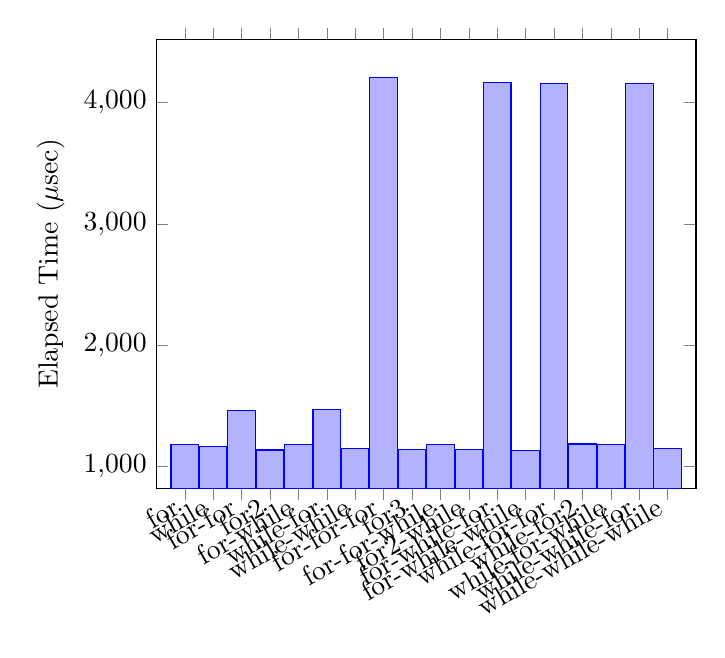
\begin{tikzpicture}
\begin{axis}[ybar,
  x tick label style={rotate=30, anchor=east},
  ylabel=Elapsed Time ($\mu$sec),
  xmin=0, xmax=19,
  xtick={1,2,3,4,5,6,7,8,9,10,11,12,13,14,15,16,17,18},
  xticklabels={for, while, for-for, for2, for-while, while-for,
  while-while, for-for-for, for3, for-for-while, for2-while,
  for-while-for, for-while-while, while-for-for, while-for2, while-for-while,
  while-while-for, while-while-while}]
\addplot coordinates
{(1, 1183) (2, 1166.2) (3, 1464)  (4, 1135.4) (5, 1183) 
 (6, 1467.8) (7, 1145.2) (8, 4209.6) 
 (9, 1136.4) (10, 1182) (11, 1136)
 (12, 4165.6) (13, 1129.4) (14, 4156)
 (15, 1184.8) (16, 1179.4) (17, 4155)
 (18, 1144.6)};
\end{axis}
\end{tikzpicture}
